\newpage
\section{Anhang}
\begin{figure}[h]
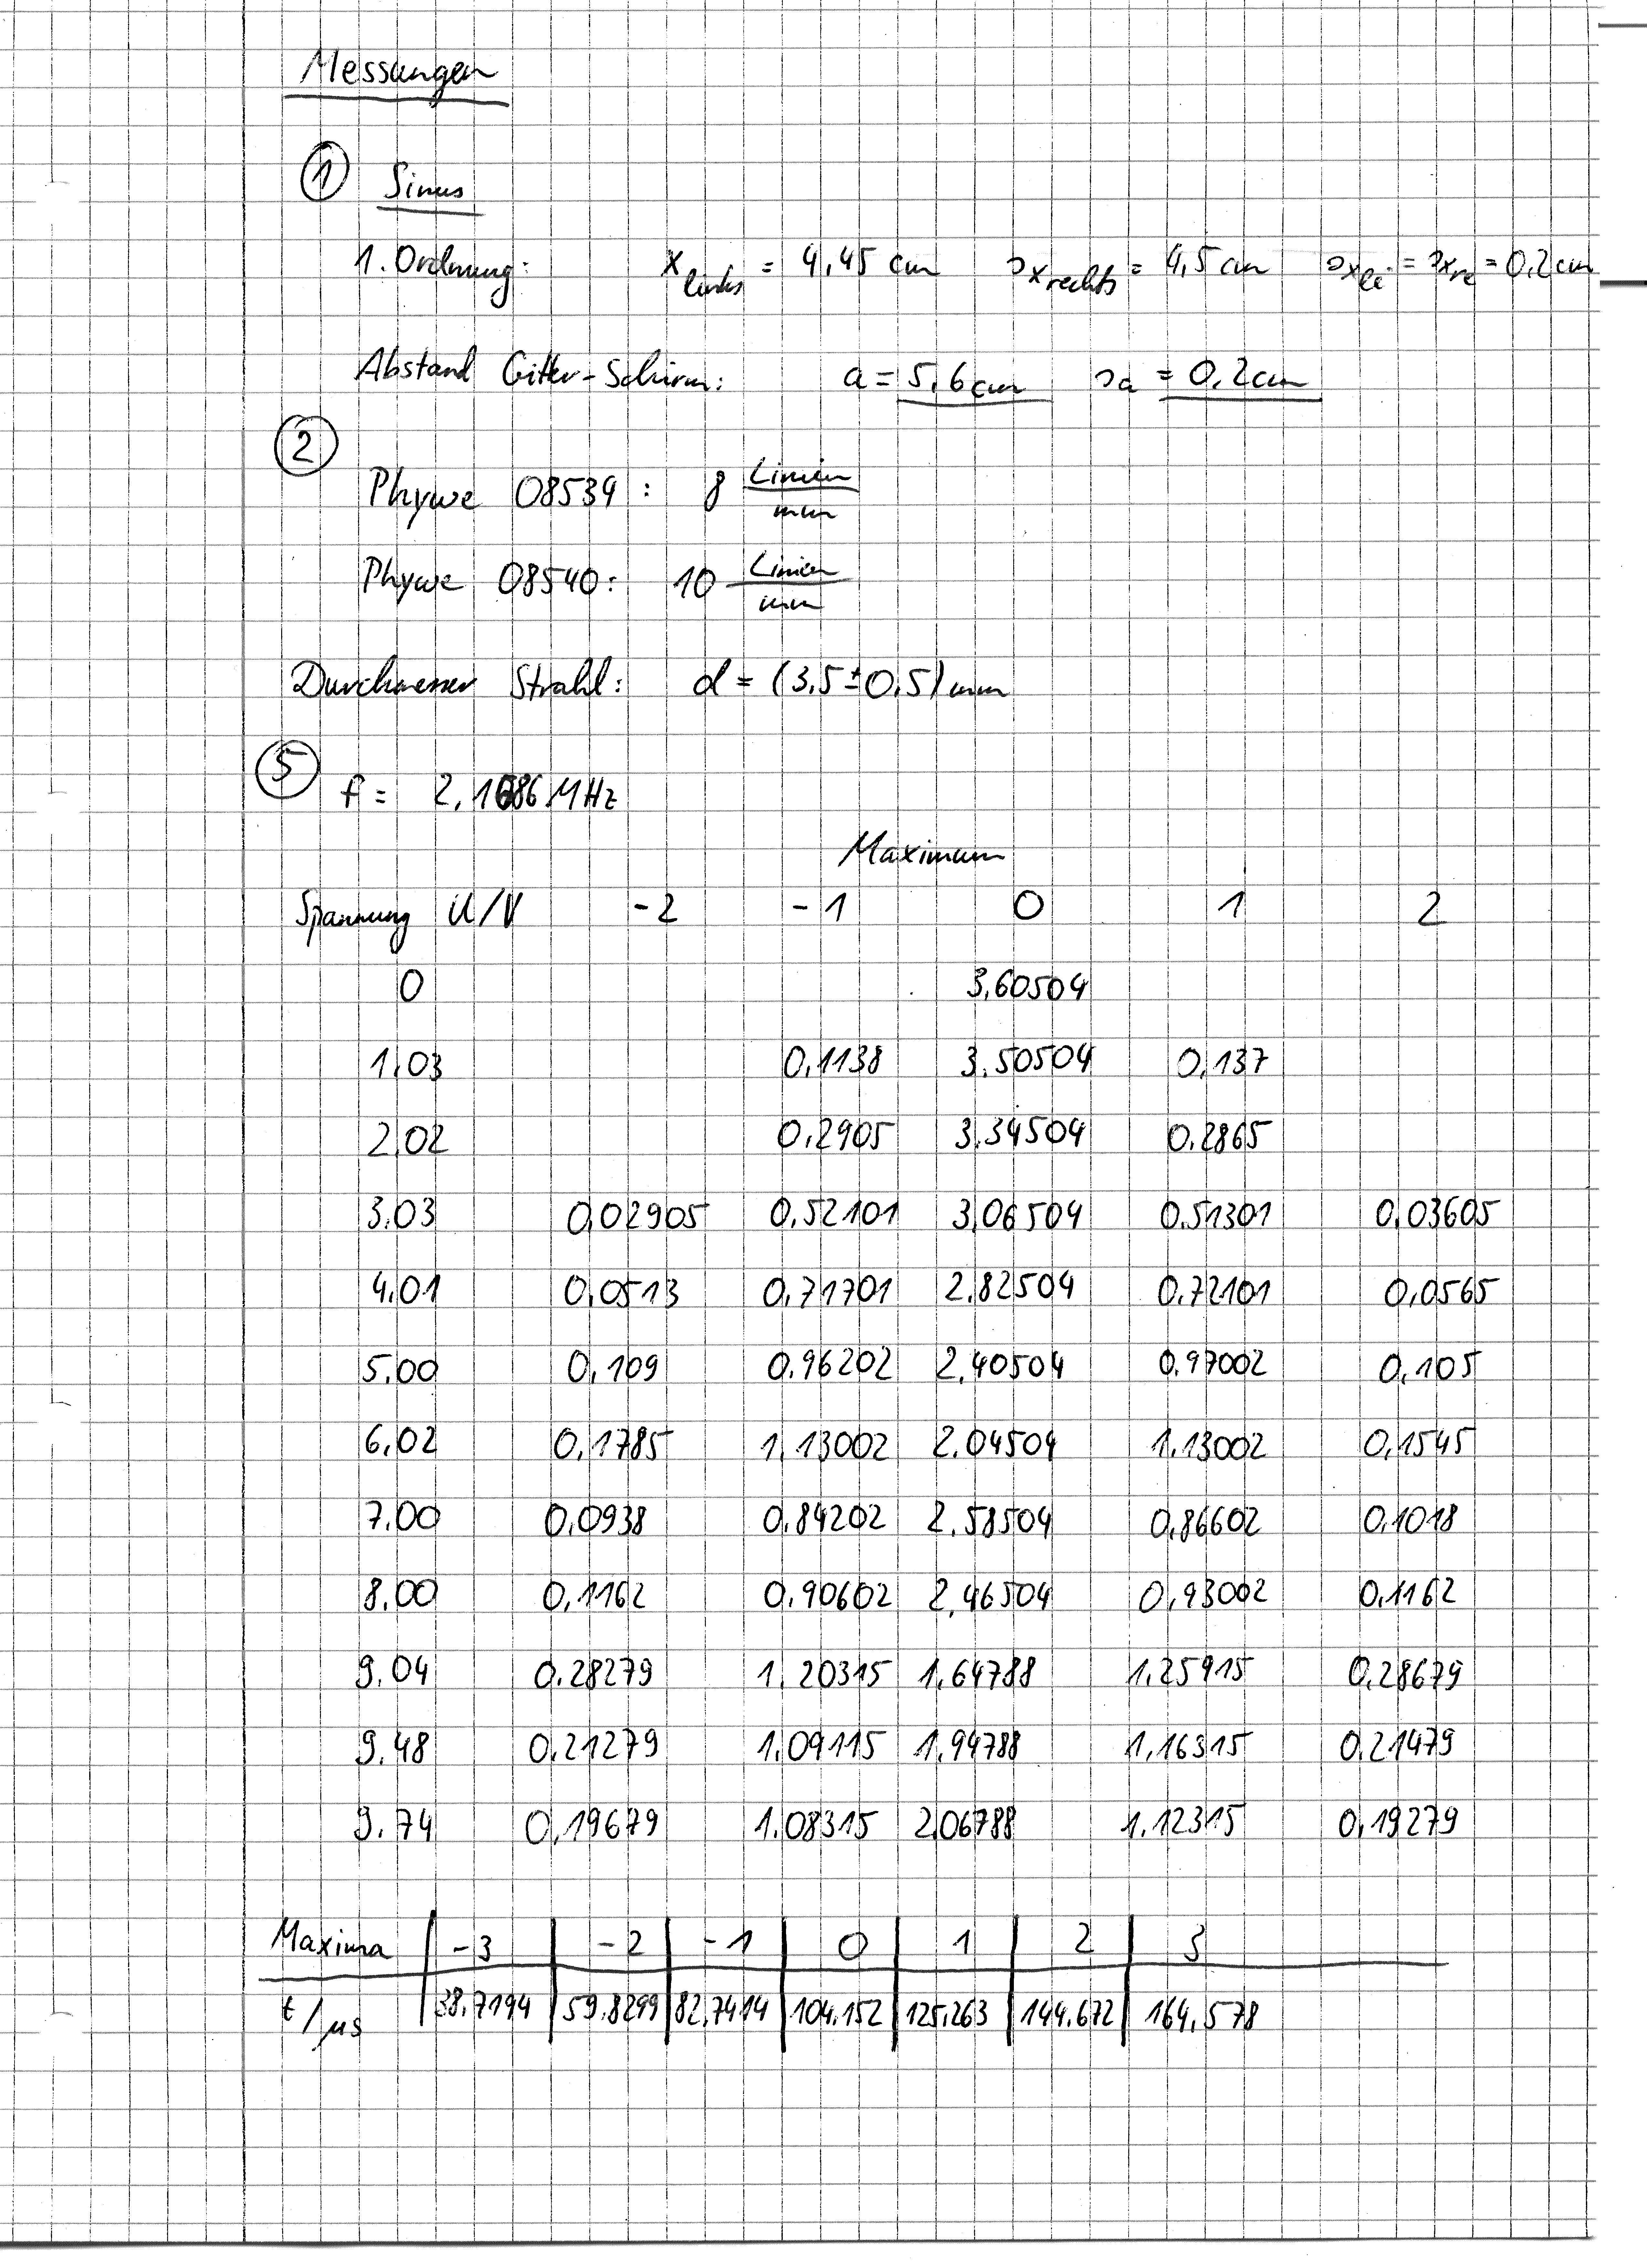
\includegraphics[scale=0.17]{anhang1}
\caption{Messung zum Faraday-Effekt.}
\label{fig:anhang1}
\end{figure}
\clearpage
\begin{figure}[h]
\begin{center}
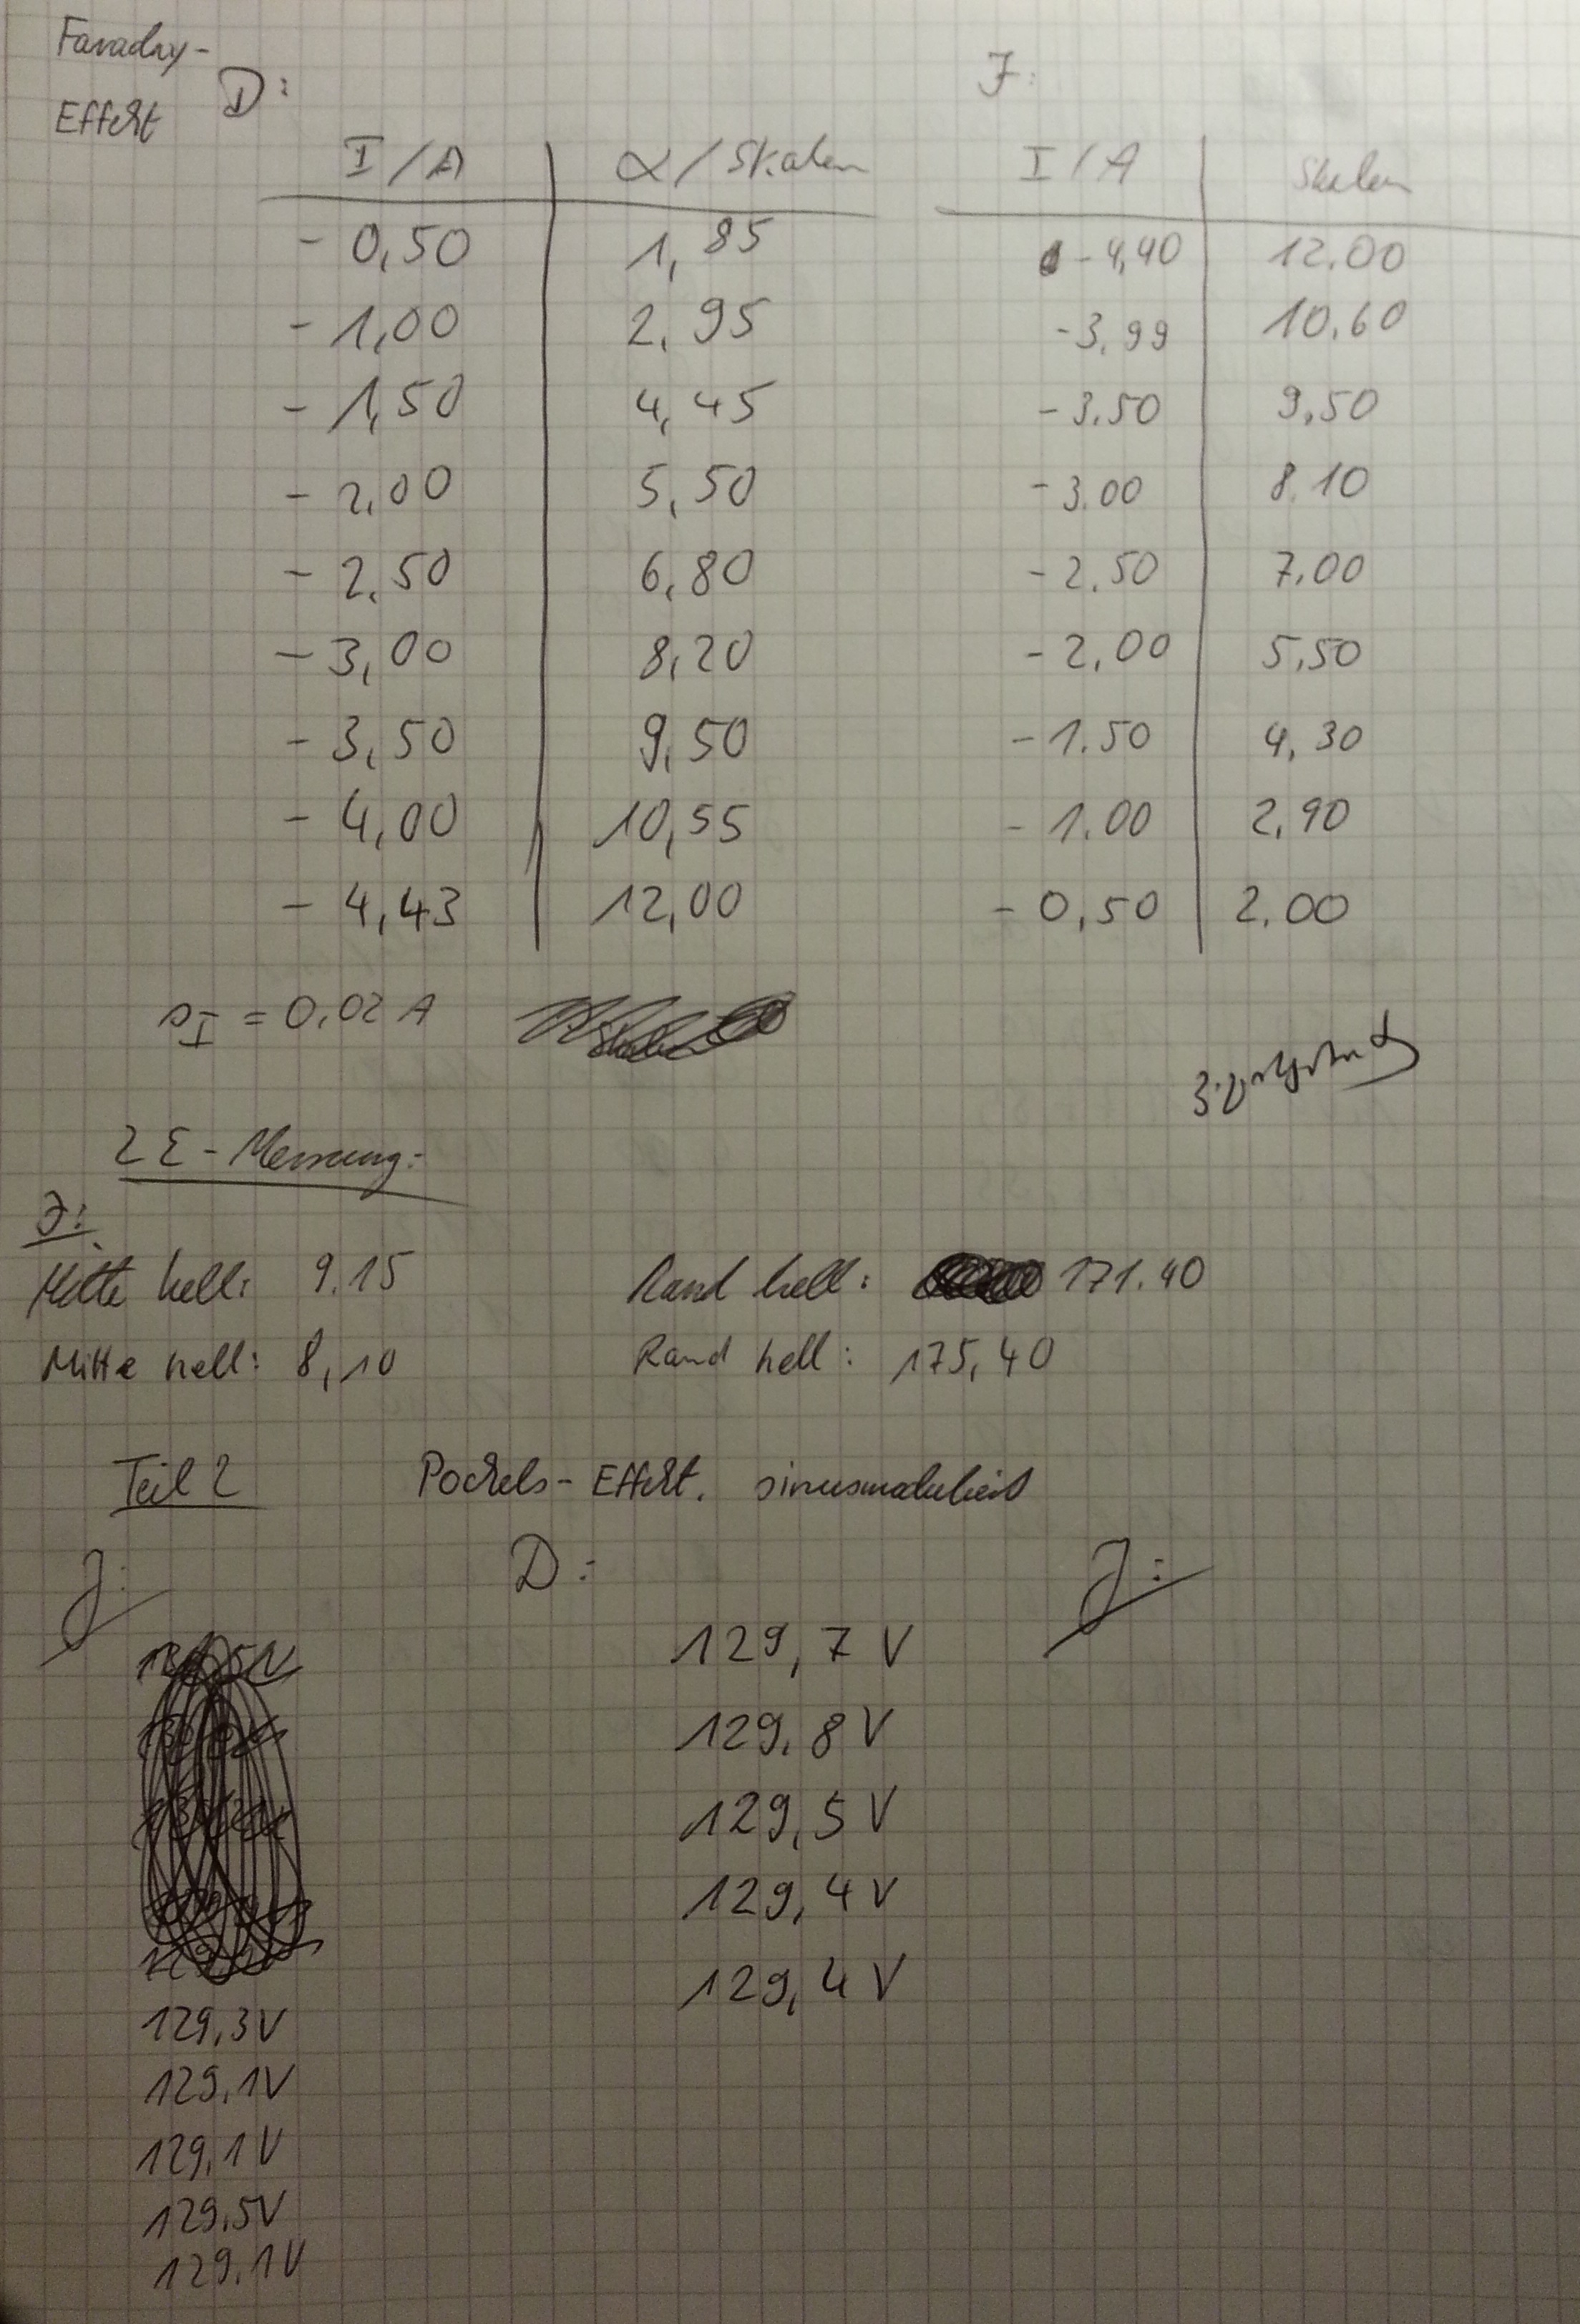
\includegraphics[scale=0.2]{anhang2}
\caption{Messung zum Faraday-Effekt und Pockels}
\label{fig:anhang2}
\end{center}
\end{figure}
\clearpage
\begin{figure}[t]
\begin{center}
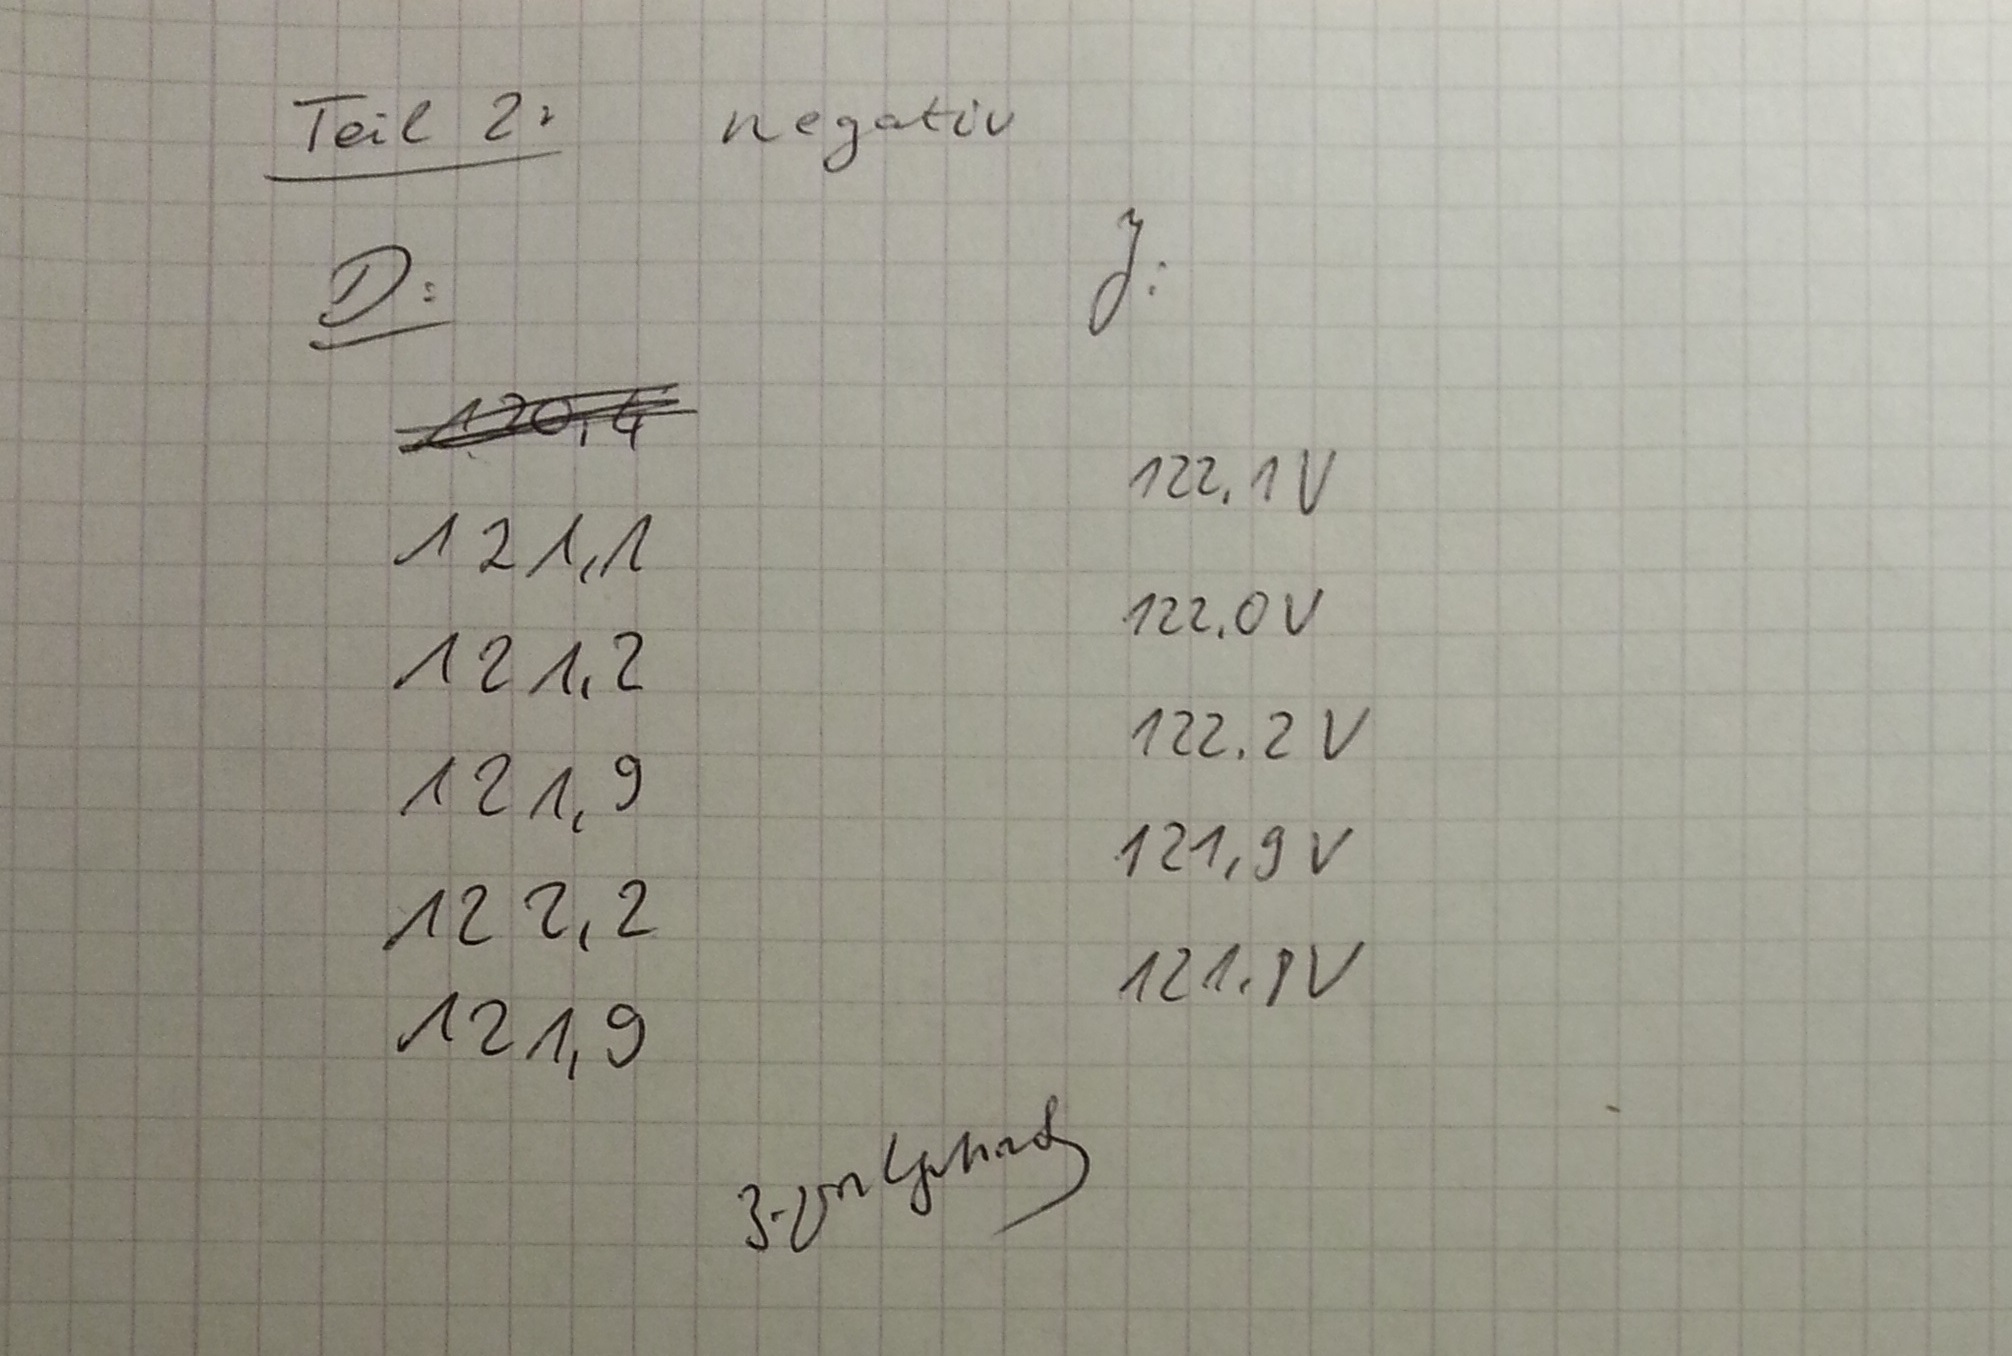
\includegraphics[scale=0.2]{anhang3}
\caption{Messung zum Pockelseffekt}
\label{fig:anhang3}
\end{center}
\end{figure}